\chapter{Introduction}
\label{chap:introduction}

Despite technological advances in the past fifteen years, genome sequencing (determining the DNA sequence of an organism) remains a challenging task. With the current technology it is not possible to ”read” the DNA sequence in one
piece from the beginning to the end. Instead, relatively short fragments must
be sequenced individually and then painstakingly assembled into the complete
sequence. This is a very laborous and expensive process, complicated by the fact
that large proportion of most genomes consists of repetitive sequences. Therefore,
instead of the pure de novo approach of assembling the complete sequence from
scratch, most of the sequencing done today merely aims to determine differences
between the sequenced organism and a complete, gold standard reference genome obtained previously by other means. This approach is known as \textif{resequencing} and is, comparatively, a much simpler task.

The most widely used sequencing platform today is Illumina and the algorithms developed in this work assume Illumina data on input. The platform takes advantage of massive parallelism, where an ensemble of DNA molecules is fragmented into very short pieces (usually ∼500 bp) and then sequenced in parallel from both ends. In one sequencing run, more than $10^9$ of short sequences are obtained simultaneously. These sequences are called \textif{reads}. Due to technical limitations, reads are only ∼150 bp long, but when they are mapped to the reference genome, many will overlap and cover the whole genome, thus enabling to determine the differences between the sequenced organism, such as single nucleotide polymorphisms (SNPs) or short insertions and deletions (indels). Collectively, these differences are refered to as \textit{variants} and the process of determining the variants is known as \textif{variant calling}.

[show IGV snapshot - what alignment looks like, with a SNP and an indel]

In order to distinguish between random sequencing errors and real variants, we need sufficient coverage (the average number of reads mapped to a position of
the genome). Thus for variant calling we need first to confidently place the reads
to the correct location of the genome (the problem known as \textif{mapping}), correctly determine the exact sequence of matches, mismatches, insertions and deletions at the location (\textit{alignment}) and finally apply a statistical model to tell appart true variation from random sequencing errors, mapping errors and alignment errors (variant cal ling).

Single nucleotide variants are easier to call, indels are more problematic. This is partly because reads containing indels can be often aligned in multiple ways,
leading to ambigous alignments and false calls, especially in difficult parts of
the genome of low complexity or high repeat content. 

\section{Basic Terms}
\label{sec:basic-terms}

For the rest of this thesis, a genome is viewed as a string of character, each represents a nucleotide, at certain position. Since DNA molecules consist of four types of nucleotides, only four characters, \texttt{A}, \texttt{C}, \texttt{G} or \texttt{T}, appear in the string. The four nucleotides have similar chemical structure. They are composed of a sugar molecule and a posphate group, which are identical for all four of them, and a unique nitrogenous base. Hence the term \textit{base} is often used when referring to a nucleotide at a specific position. Each of the bases pairs with one other, \texttt{A} with \texttt{T} and \texttt{C} with \texttt{G}, therefore knowing the sequence of one strand of a DNA double helix determines the sequence of the complementary strand. Hence the terms \textit{base pair} and \textit{base} are used interchangeably.

The algorithm developed and discussed in this work expect a large bunch of short reads on input. It expects that the sequenced organism and the reference genome are similar enough to, so an assumption that reads are correctly mapped can be made. Its task is to resolve local differences arising from incorrect read alignments. This is a subproblem of the assembly one, called \textit{microassembly}.

Some assembly algorithm transform each read into a sequence of \textit{k-mers}, substrings of equal length, usually named $k$. The read sequence of length $l$ is decomposed into $l - k + 1$ k-mers $k_0, ..., k_{l-k}$ of length $k$. If we denote bases in the read as $b_0, ..., b_{l-1}$, the k-mer $k_i$ covers bases from $b_i$ to $b_{i+k-1}$. Such definition implies that adjacent k-mers overlap by $k-1$ bases. 

An example of transforming e sequence \texttt{TACTGGCC} into k-mers of length $3$ is ilustrated on Figure \ref{fig:seq-division}. The sequence has $8$ bases in length and $6$ k-mers are created from it. The read sequence, as in all other figures in this work, is marked red, contents of individual k-mers is in yellow.

\begin{figure}[h]
	\centering
	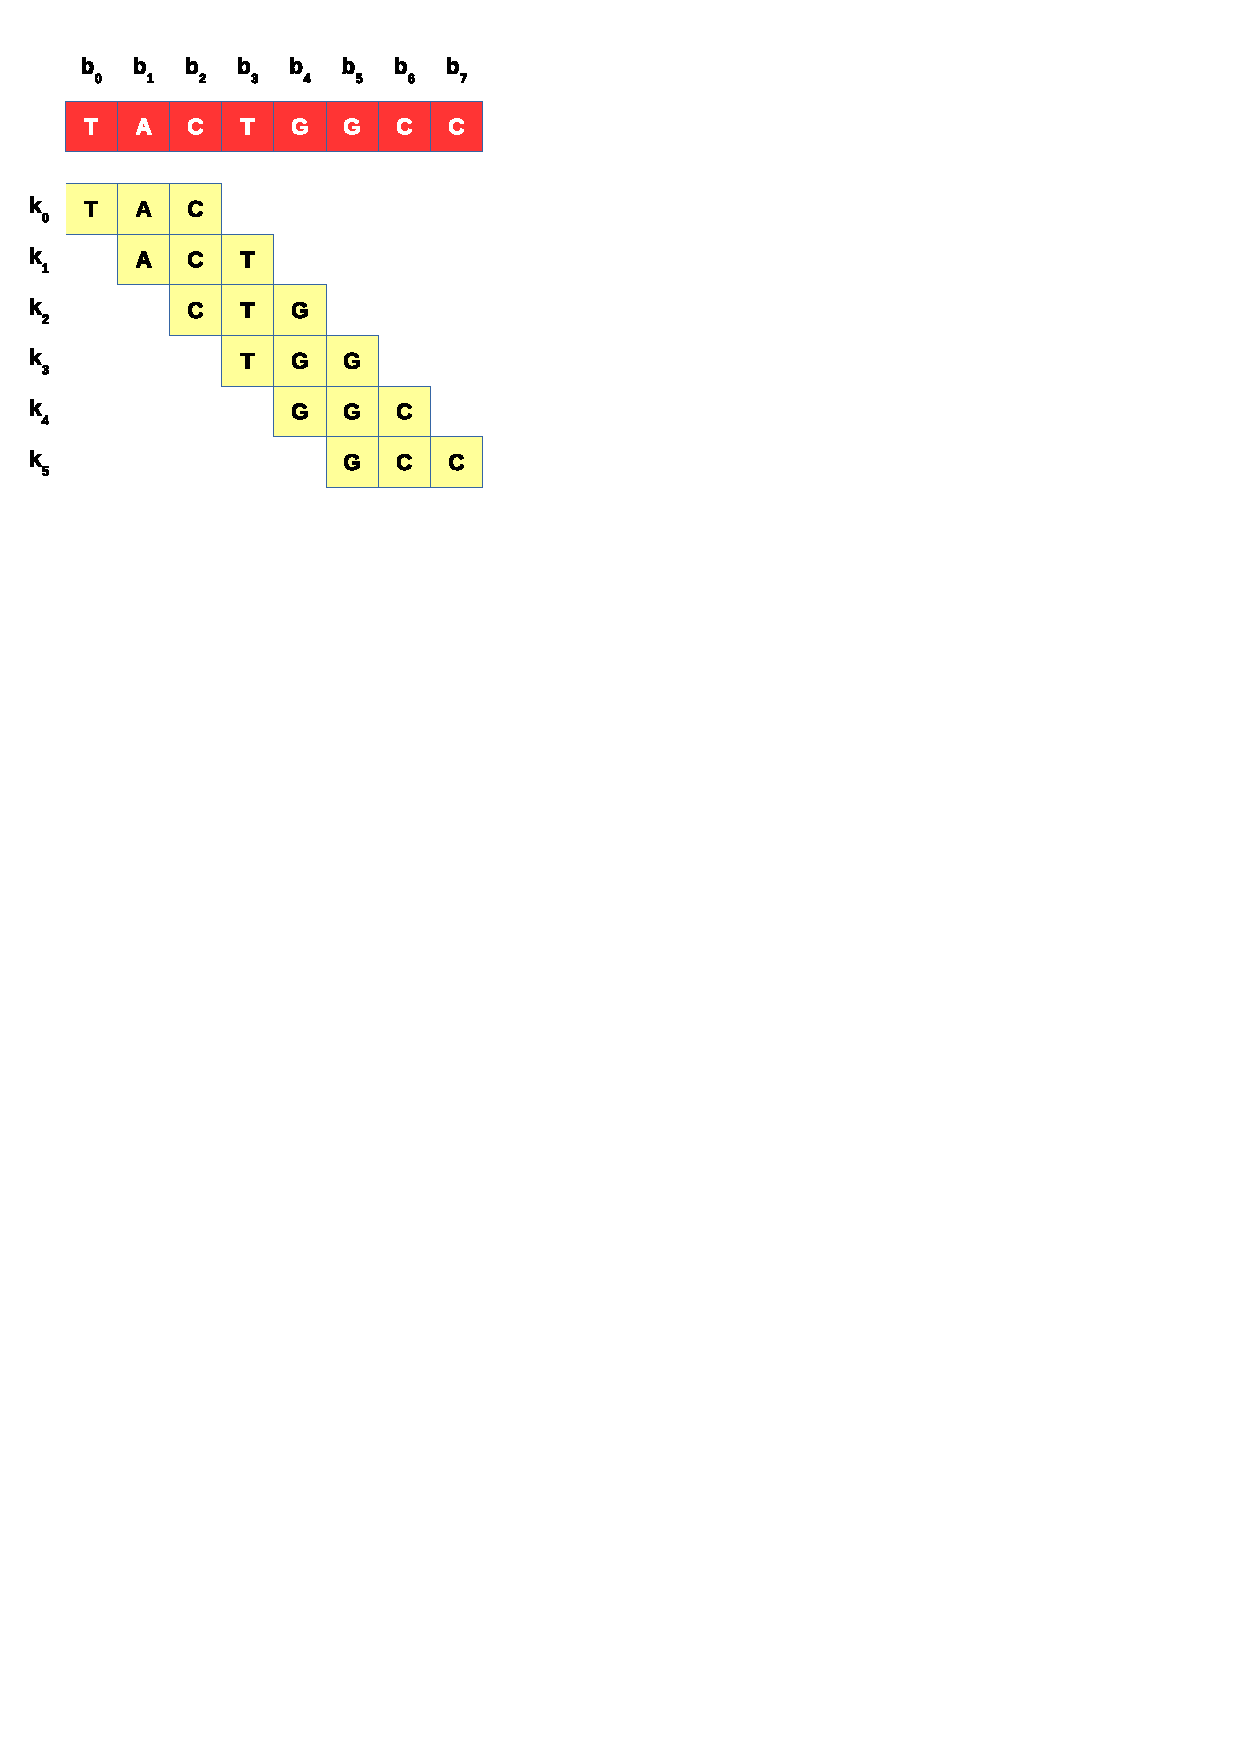
\includegraphics{img/seq-division.pdf}
	\caption{Sequence transformation into k-mers}
	\label{fig:seq-division}
\end{figure}

\section{The Model}
\label{sec:the-model}

The simplest mathematical assembly model, assumes that we are assembling genome string of length $g$, given a set of $n$ reads of length $l$ ($l << g$), each potentialy transformed into a sequence of $l-k+1$ k-mers. The model assumes that bases are, from the genome string, sampled uniformly and randomly and that no errors were produced during the sampling (in other words, all reads contain no misread bases). Since the probability of sampling a base at certain genome position is very low for single sampling event, and the number of sampling events is quite large, the problem of genome base coverage depth (i.e. number of times each base in the genome string appears in reads) follows a Poisson distribution. In other words, the probability that base at certain position is sampled $k$ times is
$$
\frac{c^k}{k!}*e^{-c}
$$
$c$ is a base coverage depth, also known as sequencing depth, and can be computed simply as a total number of bases within the input read set divided by the length of the genome.
$$
c = \frac{n * l}{g}
$$
Very similar relations apply for k-mer coverage depth, only the formula for the k-mer coverage depth needs to be changed to $\frac{n*(l - k + 1)}{g - k + 1}$. These details brings answers to at least two important problems: how many reads need to be created to (statistically) cover the whole genome string, and how to determine whether a given read set is free of sequencing errors?

The percentage of genome not covered by any read from the set is equal to $P(k=0) = e^{-c}$. Multiplying it by the genome size $g$ gives us the number of uncovered bases. So, to cover the whole genome, this number must be lower than $1$ which places condition of $c > ln g$. For example, to cover the whole human genome ($g = 3 * 10^9$), the read coverage depth must be at least $22$. 

Solution to the second problem is implied by the facts that k-mer coverage of the genome follows a Poisson distribution, and that all the theory above was made with an assumption of no sequencing errors. In an ideal case, the k-mer frequency distribution function of an error-free read set would follow the probability mass function of the Poisson distribution, meaning that frequencies of most of the k-mers are near the k-mer coverage depth. However, when we introduce possibility of sequencing errors, it happens that some k-mers would be sampled less often and some become even unique. The k-mer frequency distribution of such a read set does not follow the Poisson distribution. The aspect of sequencing errors and their means of their correction are described in great detail in Chapter \ref{chap:read-error-correction}.

\section{The Real World}
\label{sec:real-world}

One of the main differences between the ideal and real sequencing data lies in the fact that the real one contain sequencing errors. In other words, some of the reads contain incorrectly interpreted bases. To help with identifying such bases, each base of a read has its \textit{base quality}, a probability that the given base is incorrect. Base qualities are usually represented as single small numbers $q$ and the following formula is used to compute the actual error probabilities:
$$
P(base is wrong) = 10^{-\frac{q}{10}}
$$
For read sets stroed using a text format, such as SAM or FASTQ, each base quality is encoded as a single ANSI character. Since the first 32 characters of the ASCII table are not printable, and the space character is coded by $32$, the base quality values are incremented by $33$. When loading the reads from such a text format, the bias need to be taken into account. 

Also, a read may be accompanied by information about its position within and alignment to the reference sequence. Similarly to the base quality case, these information should not be taken as hard facts. The position information (also referred to as \textit{mapping position}) has also its quality (\textit{mapping quality}) following the same rules as base qualities. Although the position information may be wrong, it may help us in cases when we are interested only in assembling justa part of the genome and would like to filter out reads that do not fall within our region.

The read alignment information are given in form of a CIGAR string that describes how the source of the read set thinks individual bases of the read map to the reference. The string is formatted as a set of numbers defining sequence lengths, each followed by one character describing the alignemnt operation. The most common operations include:
\begin{itemize}
\item \textbf{Match (M)}. The base sequence matches exactly the corresponding reference bases.
\item \textbf{Mismatch (X)}. The sequence is aligned to certain part of the reference but the corresponding bases differ.
\item \textbf{Insertion (I)}. The sequence is inserted to the reference at a given position. Then, the read continues to follow the reference at this position plus one.
\item \textbf{Deletion (D)}. The read sequence skips the corresponding part of the reference.
\item \textbf{Hard-clip (H)}. 
\item \textbf{Soft-clip (S)}. The sequence does not match the corresponding reference at all. The situation may occur only on the beginning and an end of the read.
\end{itemize}

For example, assume a reference \texttt{CAGGTGTCTGA} and a read GGTGAATCTA with the following alignment:
\begin{verbatim}
           1 2 3 4 5 6     7 8 9 A B
Reference: C A G G T G     T C T G A
Read:          G G T G A A T C T   A
\end{verbatim}
The read starts at reference position 3 and the alignment can be represented as the \texttt{4M2I3M1D1M} CIGAR string.

Genomes of diploid organisms, introduce another problem not covered by the simple mathematical model covered earlier. Since such organism owns two sets of chromosomes (one from each of its parents), both sets are present within the read set obtained by chopping the genome to short reads. That implies that two genome strings are present within, and need to be reconstructed, from the input read set.

\section{Major Assembly Algorithm Classes}
\label{sec:major-assembly-algorithm-classes}

Currently, there are two widely used classes of algorithms: overlap-layout-consensus (OLC) and de-bruijn-graph (DBG) \cite{alg-compare}. Algorithms belonging to the former base their idea on constructing a graph recording overlapping reads and extracting the alternate sequences from it. Main idea behind the DBG class is to chop all reads into k-mers that are then uses to construct a de Bruijn graph which is, after some optimizations, is subject to derivations of alternate sequences.

\subsection{De Bruijn Graphs}
\label{subsec:de-bruijn-graphs}

De Bruijn graphs (DBG) were originally invented as an answer to the superstring problem  (finding a shortest circular string containing all possible substrings of length $k$ (k-mers) over a given alphabet) \cite{dbg-apply}. For a given $k$, de Bruijn graph is constructed by creating vertices representing all strings of length $k-1$, one per string. Two vertices are connected with a directed edge if there exist a k-mer such that the source and destination vertices represent its prefix and suffix of length $k-1$ respectively. The k-mer labels the edge. 

Formally, let $L_k$ be a language containing all words of length $k$ over an alphabet $\sigma$, then de Bruijn graph $B(V, E)$ is defined as
\begin{gather}
V = \{v_w | w \in L_{k-1}\} \\
E = \{(v_u, v_w) | x \in L_k,  u is its prefix and w its suffix \} \\
\end{gather}
The shortest superstring is found by concatenating all $k-1$-mers represented by vertices on any Eulerian cycle of the corresponding de Bruijn graph. Since a polynomial-time algorithm for finding an Eulerian cycle is known, the superstring problem can be effectively solved.

\subsubsection{Application to Genome Assembly}
\label{subsub:dbg-application-to-genome-assembly}

SImilarly, de Bruijn graphs can be used for genome assembly, especially if the genome question is circular. Assume that, for a fixed $k$, all k-mers of the target genome are known. Then a DBG can be constructred in two different ways:
\begin{itemize}
\item \textbf{K-mers are represented by edges}. Each edge is labelled by a k-mer in the same way as in the graph used for solving the superstring problem. Each edge connects vertices representing (k-1)-mers forming prefix and suffix of its k-mer. The genome string can be reconstructed by choosing the right one from all possible Eulerian cycles. This approach is presented and discussed in \cite{dbg-apply}.
\item \textbf{K-mers are represented by vertices}. Each k-mer is represented as a single vertex. Edges reflect the k-mer order within reads. To recover the genome, one needs to find a Hamiltonian path of the graph, which is one of NP-complete. problems. Among others, HaploCall \cite{haplocall} used by GATK takes advantage of this way of de Bruijn graph usage.
\end{itemize}

\subsubsection{HaploCall}
\label{subsub:haplocall}

Rather than assembling whole genome at once, HaploCall starts with detection of regions that are likely to contain variants. A score is computed for every genome position, reflecting the probability of variant occurrence. Regions are formed around positions classified as interesting. As subset of the input reads is assigned to each of the regions; reads are selected based on their mapping position. Each region is then processed separately and independently of others.

The active region processing phase starts by decomposing the reference sequence covering the region into k-mers and using them as vertices in a newly constructed de Bruijn graph. Edges connect vertices representing k-mers adjacent by their position within the reference. For each edge, a weight value is initialized to zero.

When the reference is transformed into the graph, a similar process happen with each of the input reads assigned to the active region. The read is decomposed into k-mers that are inserted into the graph in the same manner as the reference k-mers. Again, edges follow the order of k-mers within reads.  New vertices are created only for k-mers not seen in the reference, similar case applies to new edges --- if an edge denoting adjacent position of two k-mers already exists, its weight is increased by one. Otherwise, a new edge with weight initialized to $1$ is inserted into the graph. The weight values actually count number of reads covering individual edges.

After inserting all the reads into the graph (the HaploCall documentation refers to the step as Threading reads through the graph), it is time to simplify the graph structure a little bit. The main concern here is to remove graph sections created due to sequencing errors present in the input reads. Such sections are identified by their low read coverage and removed. Other structure refinements are performed, including removal of paths not leading to the reference end.

In the next stage, most probable sequences are extracted from the resulting graph. Each sequence is represented by a path leading from the starting k-mer of the reference to ending one and its probability score is computed as the product of so-called transition probabilities of the path edges. Transition probability of an edge is computed as its weight divided by the by the sum of weights of all edges sharing the same source vertex. By default, 128 most probable paths are selected.

The Smith-Waterman algorithm is used to align each of the selected sequences to the reference. The alignment is retrieved in form of a CIGAR string that indicates places of possible variants, such as SNPs and indels. Indel positions are normalized (left aligned). 

The CIGAR strings actually contain a super set of the final set of called variants. To filter out false positives, other solutions are employed (for example, the HaploCall documentation mentions UnifiedGenotyper for GATK).

\subsection{Overlap-Layout-Consensus}
\label{subsec:overlap-layout-consensus}

Algorithms taking advantage of this approach usually do not decompose reads into k-mer sequences. Reads are considered to be the smallset units. As the name suggests, the work is done in three steps.

Main purpose of the overlap phase is, not surprisingly, to compute overlaps between all possible pairs of the input reads. Since number of short reads within high coverage data sets may go to milions, the process of overlap computation may take a lot of processor and memory resources. Overlapping reads are connected into longer seuqnces called \textit{contigs}. Actually, a graph is being constructed, its vertices represents individual reads (or contigs) and edges represent overlaps.

The definition of read overlapping is not strict. Two reads are considered overlapping (and thus, are connected by an edge) if they overlap at least by $t$ bases, allowing several mismatches. The constant $t$ is a parameter of the algorithm and is called a \textit{cutoff}.

During the \textit{layout} phase, a read-pairing information is used to put disconnected parts of the read overlapping graph together and resolving structures created by sequencing errors. The \textit{consensus} phase is responsible for deriving candidate seuqnces for variant calling from the graph. In an ideal case, the cadidate sequences would be the Hamiltonian apths of the graph.

\section{Goals of this Work}
\label{sec:goals-of-this-work}

Main goal of this work is to develop an algorithm capable of variant calling on high-thorought data sets, comparable to, or more precies than methods currenlty employed. The approach used by HaplotypeCaller (HaploCall) should be used as an inspiration which implies the newly developed algorithm would take advantage of the reference sequence and would belong to the class of algorithms utilizing de Bruijn graphs.

The new algorithm should accept the input data set in widely used formats, such as SAM for the read set and FASTA for the reference sequence, and output the called variants in the VCF format. Its results need to be compared to at least two other assembly and variant calling tools. GATK (HaploCall) \cite{haplocall}, as a representative of the DBG class and reference-aided methods, and FermiKit \cite{fermikit}, utilizing the OLC concept.